%-/`-/`-/`-/`-/`-/`-/`-/`-/`-/`-/`-/`-/`-/`-/`-/`-/`-/`-%
% CS 196 Copyrights and Patents Survey
% 
% Typeset with the `acmlarge` template by Donald Knuth & Leslie Lamport
% 
% Copyright 2016 Fiestada, Lobaton, Dacuba, Cañedo, Latoga
% For more information about this survey, go to https://cs196copyrights.github.io/survey
% or email the Git repo maintainer at vffiestada@up.edu.ph
%
%-/`-/`-/`-/`-/`-/`-/`-/`-/`-/`-/`-/`-/`-/`-/`-/`-/`-/`-%
\documentclass[prodmode,cs196]{acmlarge}

\usepackage{float}

% Metadata Information
\acmVolume{1}
\acmNumber{1}
\acmArticle{2}
\articleSeq{1}
\acmYear{2016}
\acmMonth{09}

% Page heads
\markboth{Ca\~{n}edo, Dacuba, Fiestada, Latoga, and Lobaton}{Opinions of UP Diliman Students on Technology Copyrights and Patents}

% Title portion
\title{Opinions of UP Diliman Students on Technology Copyrights and Patents}
\author{ABBY CA\~{N}EDO, CARISSE DACUBA, VINCENT FIESTADA, AREL LATOGA, and TROI LOBATON \affil{University of the Philippines Diliman}}

\begin{abstract}
In this paper, the authors take a look at the popular opinion of Science and Engineering majors in the University of the Philippines Diliman Students regarding isssues around technological copyrights and patents. In particular, this paper examines their opinions on the extent of influence that a particular piece of design or feature has on a whole product. This is done in the context of the Samsung vs. Apple and Oracle vs. Google trials over the infringement of intellectual property rights.
\end{abstract}

\category{Ethical and Professional Issues}{Technology and Computing}{Popular views and opinions}[Surveys and Analyses]

\terms{Patents \and Copyrights}
\keywords{Ethics, patents, copyrights, technology, computing}

\acmformat{Ca\~{n}edo, Dacuba, Fiestada, Latoga, and Lobaton. 2016. Opinions of UP Diliman students on technology copyrights and patents.}

\begin{document}

\begin{bottomstuff}
\copyright Copyright 2016 Ca\~{n}edo, Dacuba, Fiestada, Latoga, and Lobaton.
\end{bottomstuff}


\maketitle

\section{Introduction}

Technological patents and copyrights pose an important issue for software developers, hardware manufacturers, designers, and other stakeholders in the technology industry and those communities concerned about technological proliferation. These issues raise questions about how much control an entity should have over its creation, what protections should be afforded that entity, and how those protections should be balanced to still allow continued innovation in the field. Furthermore, how much influence does a particular piece of design or technology have over a product? 

\subsection{Intellectual Property Rights}

Intellectual property (IP) such as art, designs, and inventions are identified as non-physical works that are the "product of original thought". Rights can be granted to the owners of IP. These rights cover the control of the expressions of IP (such as physical expressions in the form of manufactured products, or digital copies of a work of art or piece of technology). Intellectual property rights protects the interests of the creator by giving them control over the production and distribution of expressions of their work. \cite{MooreHimmaIP} Protections can be granted by law in the form trademarks, trade secrets, patents, and copyrights. This paper is concerned with the latter two.

A patent is a set of rights given to the owner of an invention that prevents others from making, using, importing, or selling the invention without the owner's permission. To be patented, an invention must be "new, an improvement over current processes or technologies, and must have practical industrial application". \cite{IPOSPatent} 

In general, patents expire (currently, the expire after 15 years in the US), but since the allegations discussed here fall within the time frame, a description of patent time limits can be safely ommitted. Most countries grant patents to several types of intellectual property. This paper is generally concerned with design and utility patents. 

In the United States, where the Apple patents were filed, a design patent can be applied for the ornamental or aesthetic design of a product, including its physical properties and appearance. Patents last for 15 years in the US and allows its holder to disallow the unauthorized use, marketing, or selling of a design. \cite{USPTOPatents}

A utility patent is one granted to a useful and novel, or previously unknown, process, machine, manufactured product, or composition of matter. These include the patent granted for Samsung's wireless technologies. \cite{USPTOPatents}

A copyright constitutes a different set of rights granted to an intellectual property owner. They are the legal rights given to the creator of works such as writings, paintings, photographs, and computer programs--i.e. expressions of ideas. Copyright prevents others from reproducing, distributing, creating derivatives from, and displaying the work in public. Another important distinction between copyright and patents is that while patents have to be applied for, copyright automatically applies to all copyrightable material. \cite{PlagiarismTodayCopyright}

\subsection{Apple vs. Samsung}

\textbf{Apple vs. Samsung} is a series of patent infringement lawsuits filed by Apple Computer, Inc. and Samsung against each other. As of the time of this writing, some cases are still pending in several courts. Apple has several design patents, including patents for the iPhone's shape, the colors of the graphical user interface of iOS, and the shape and design of the iPad.

%% Photographs from Apple's design patents
\begin{figure}[H]
	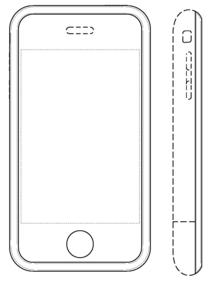
\includegraphics[width=0.3\textwidth]{apple_iphone_shape.png}
	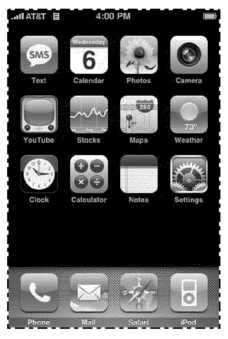
\includegraphics[width=0.3\textwidth]{apple_iphone_icons.png}
	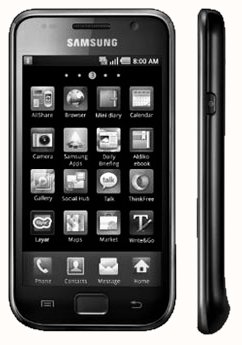
\includegraphics[width=0.3\textwidth]{samsung-galaxy-i9000.png}
	\caption{From the left: a) A front and side profile of Apple's iPhone according to the US patent grant for its design; b) A screenshot of the home screen of the iPhone showing the patented user interface; c) A front and side profile with the home screen of the Samsung Galaxy i9000, claimed by Apple to be an infringement of its design patents. }
\end{figure}

On April 15, 2011, Apple sued Samsung in the United States District Court for the Northern District of California, claiming that Samsung infringed on Apple's design patents. A few days later, on April 22, Samsung counter-sued Apple in the federal courts of Seoul, South Korea; Tokyo, Japan; and Mannheim, Germany, claiming that Apple infringed upon its own patents on wireless technology.

Apple cited the similarities between its own iPhone and iPad products and the Samsung Galaxy line of smartphones and tablets. In particular, Apple claimed infringement of US D593087 (for the "home button, rounded corners, and tapered edges" of the iPhone); \cite{AppleiPhoneDesignPatent}

\section{Methodology}

\label{sect:bib}
\bibliographystyle{acmref}
\bibliography{report_sources}{}

\end{document}